\documentclass[tikz]{standalone}
\begin{document}

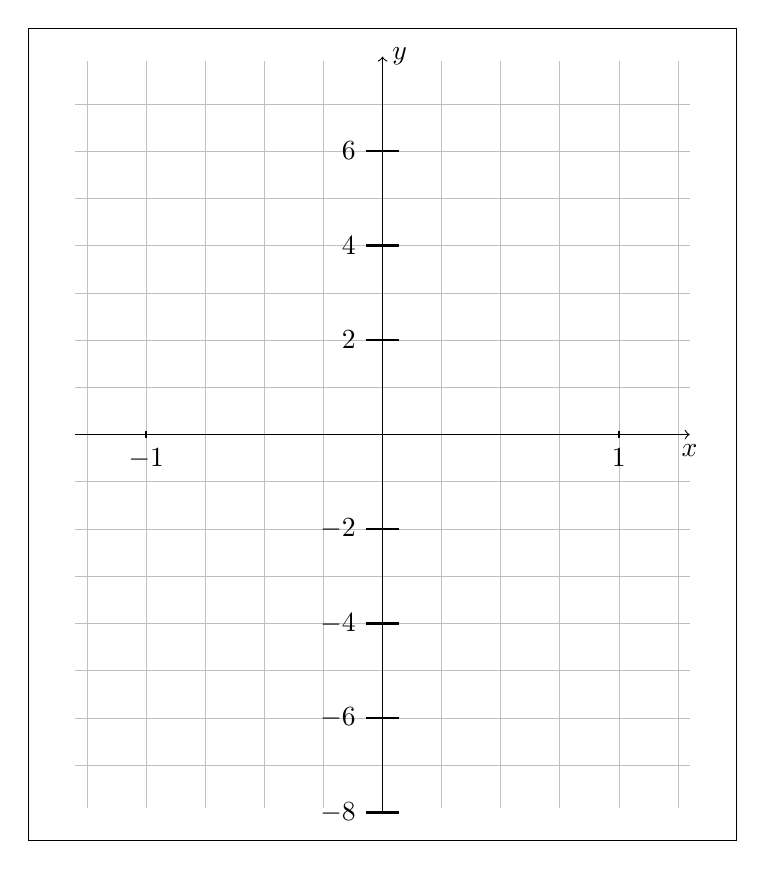
\begin{tikzpicture}[xscale=3,yscale=0.6]

\draw[black,fill=white] (-1.5,-8.6) rectangle (1.5,8.6);
\draw[very thin,color=lightgray,ystep=1,xstep=0.25] (-1.3,-7.9) grid (1.3,7.9);

      \draw[->] (-1.3,0) -- (1.3,0) node[below] {$x$};
      \draw[->] (0,-8) -- (0,8) node[right] {$y$};
%\draw[domain=-1:1,smooth,variable=\x,black,ultra thick,samples=100] plot ({\x},12*\x*\x-\x-6);
       
      % tick marks
\foreach \x in {-1,1} 
	\draw [thick] (\x cm,2pt) -- (\x cm,-2pt) node[below] {$\x$};
\foreach \y in {-8,-6,-4,-2,2,4,6} 
	\draw [thick] (2pt,\y cm) -- (-2pt,\y cm) node[left] {$\y$};

    \end{tikzpicture}
\end{document}
